% IEEE Conference Paper - FormSathi
% Compiled with: pdflatex research-paper.tex
\documentclass[conference]{IEEEtran}

\IEEEoverridecommandlockouts

\usepackage{cite}
\usepackage{amsmath,amssymb,amsfonts}
\usepackage{algorithmic}
\usepackage{graphicx}
\usepackage{textcomp}
\usepackage{xcolor}
\usepackage{booktabs}
\usepackage{multirow}
\usepackage{tabularx}
\usepackage{url}
\usepackage{hyperref}
\usepackage{tikz}
\usetikzlibrary{arrows.meta, positioning, shapes.geometric, fit, calc}
\def\BibTeX{{\rm B\kern-.05em{\sc i\kern-.025em b}\kern-.08em
    T\kern-.1667em\lower.7ex\hbox{E}\kern-.125emX}}

\begin{document}

\title{FormSathi: An AI-Powered Multilingual Form Assistant Using Computer Vision and Retrieval-Augmented Generation}

\author{
  \IEEEauthorblockN{Aryan Singh Tomar\IEEEauthorrefmark{1},\;
                    Sri Krishna\IEEEauthorrefmark{2},\;
                    Sushruth V Kamble\IEEEauthorrefmark{3}}
  \IEEEauthorblockA{%
    \IEEEauthorrefmark{1}\IEEEauthorrefmark{2}\IEEEauthorrefmark{3}%
    School of Computer Science and Engineering, RV University}
}

\maketitle

% ------------------------------------------------------------------
\begin{abstract}
It can be challenging for a person to fill out government and public service forms owing to the dense form design, domain-specific terminologies, and the presence of text written in multiple languages. In this work we propose \textbf{FormSathi}, an assistive computer vision and retrieval based system which can find fillable regions on a form page, explain field semantics, and provide text and speech guidance in English, Hindi, Kannada and Urdu. To do so for unseen forms, we utilize a multi-concept, multi-language dictionary of 56 concepts and 927 wordings, together with deterministic layout analysis; Groq-hosted generation is our external fallback system for generation and is optional. Our system does not use a local LLM. Local guidance is provided using curated knowledge, dictionary look-up and retrieval.
\end{abstract}

\begin{IEEEkeywords}
form understanding, optical character recognition, retrieval-augmented generation, multilingual NLP, computer vision, document intelligence, assistive technology
\end{IEEEkeywords}

% ------------------------------------------------------------------
\section{Introduction}

Public service forms can have dense layout, domain-specific abbreviations like \textit{EPIC}, \textit{AC Number} and \textit{IFSC}, and instructions in multiple languages. Also, scanned images and PDF annexures can represent fill-in boxes within the body of a sentence with the help of dotted leaders. The previous works on form understanding have shown that text along with page layout and field relationships are important \cite{funsd,layoutlm,formnet}, thus necessitating an explainable and multilingual approach which preserves field coordinates.

There are three kinds of existing assistive systems for filling out forms. (i) \textit{Pure OCR}: text is extracted but no semantic interpretation is provided, leaving the user clueless. (ii) \textit{Generic chatbots}: a large language model is queried about the meaning of a field name, but without looking at the page it cannot say where the answer belongs or follow the layout of the form. (iii) \textit{Form-specific parsers}: hand-coded extractors trained on one specific template which breaks the moment the form version changes.

None of these systems combine localisation (knowing \emph{where} the field is), interpretation (knowing \emph{what} it asks) and multilingual explanation (\emph{what to write} in the user's language).

\textbf{Contributions.} This paper makes the following contributions:
\begin{enumerate}
  \item Deterministic page-structure service for restoring ruled-grid tables, mapping OCR words to cells, detecting caption-and-blank overlap, finding signatures, detecting dotted-leader blanks intrinsic to PDF government forms, and blocking the suggestion of fields overlapping printed text.
  \item Multilingual field-dictionary matcher running in a three-tier fashion, tolerant to noise, working in four languages and four scripts without any external service calls.
  \item RAG pipeline running on top of per-form knowledge base and common-field dictionary with transparency in the resolution hierarchy where confidence level is indicated to the user.
  \item Privacy-preserving design never sending user-entered answers to the external LLM and transmitting answers to the backend only on user request for the preview of references.
  \item Evaluation on four seeded known forms, five identification samples of unknown-forms and eight language/quality image variants of unknown-forms; experimental results are limited to the committed evaluation artifacts.
\end{enumerate}

The rest of this paper is organized as follows. Section~\ref{sec:related} gives the survey of related works. Section~\ref{sec:system} describes system architecture. Section~\ref{sec:pagestructure} describes the page-structure service. Section~\ref{sec:understanding} describes field understanding and the multilingual guidance pipeline. Section~\ref{sec:implementation} describes the implementation. Section~\ref{sec:evaluation} describes experimental results. Section~\ref{sec:conclusion} concludes.

% ------------------------------------------------------------------
\section{Related Work}
\label{sec:related}

In the area of form understanding research, we observe a trend away from OCR and layout analysis to models that jointly represent text, image, and layout. FUNSD gives 199 annotated noisy forms and benchmarks text detection, OCR, spatial layout, and entity linking \cite{funsd}. LayoutLM combines text and layout position, and LayoutLMv3 learns multimodal text/image representations. FormNet and FormNetV2 explicitly model the structure of field relationships \cite{layoutlm,layoutlmv3,formnet,formnetv2}. Such approaches establish a strong baseline for document extraction, but they require a model to run and in themselves do not give authored explanations in the four target scripts.

OCR-free systems such as Donut combine reading and document understanding, and multilingual OCR research focuses on script-aware recognition components for document recognition across scripts \cite{donut,multilingual_ocr}. In contrast, FormSathi preserves word coordinates via OCR and relies on deterministic page geometry so that a detected answer region can be highlighted and audited. Previous work on robustness of learned field extractors highlights their sensitivity to layout and OCR perturbation, and thus motivates our testing of both clean and degraded input, while our current synthetic evaluation does not have sufficient coverage for robustness assessment \cite{form_attacks}. Interactive form-filling benchmarks have recently identified difficulties of multimodal agents to align fields to instructions, which FormSathi addresses by maintaining control of the user and avoiding automatic value submission \cite{formfactory}.

\subsection{Focused Literature Search}
\label{sec:prisma}

We provide the detailed results of a systematic literature search in PRISMA 2020 flow chart format \cite{prisma2020}; this is not an exhaustive review of all scholarly databases. The arXiv API was searched for records submitted in categories cs.CV, cs.CL, or cs.IR during the period from 2015 until the search date (4 November 2026). The six keywords were \texttt{"form understanding"}, \texttt{"multilingual OCR"}, \texttt{"form filling"}, \texttt{"OCR-free document understanding"}, \texttt{"form document information extraction"}, and \texttt{"form field extraction"}. The searches resulted in 68 records (29, 16, 14, 6, 2, and 1, respectively); all arXiv record identifiers were unique. Citation searching found an additional one study on Donut. The titles and abstracts were screened according to the scope of the document/layout, OCR, field extraction, or form-filling assistance. Nine records were reviewed in full; all nine passed the relevance screening. Thus, 60 records were excluded at title/abstract screening and nine studies included into narrative synthesis. Screening was done by one reviewer only, and this is a limitation.

\begin{figure*}[t]
\centering
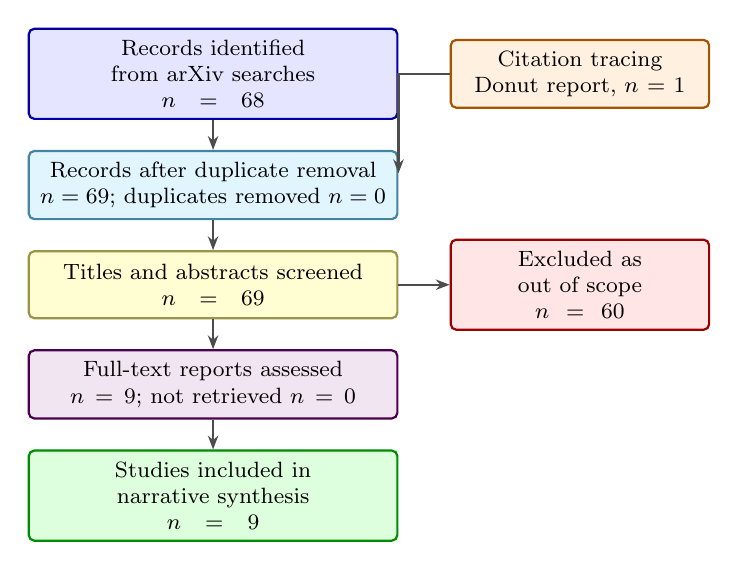
\begin{tikzpicture}[
  font=\footnotesize,
  stage/.style={draw, rounded corners=2pt, thick, align=center,
                text width=4.4cm, minimum height=0.85cm, inner sep=4pt},
  side/.style={draw, rounded corners=2pt, thick, align=center,
               text width=3.0cm, minimum height=0.72cm, inner sep=4pt,
               fill=orange!12, draw=orange!65!black},
  arrow/.style={-{Stealth[length=5pt]}, thick, draw=black!70}
]
  \node[stage, fill=blue!10, draw=blue!65!black] (identified)
    {Records identified from arXiv searches\\$n=68$};
  \node[side, right=0.65cm of identified] (other)
    {Citation tracing\\Donut report, $n=1$};
  \node[stage, fill=cyan!12, draw=cyan!60!black, below=0.38cm of identified] (dedup)
    {Records after duplicate removal\\$n=69$; duplicates removed $n=0$};
  \node[stage, fill=yellow!18, draw=yellow!55!black, below=0.38cm of dedup] (screen)
    {Titles and abstracts screened\\$n=69$};
  \node[side, right=0.65cm of screen, fill=red!10, draw=red!60!black] (excluded)
    {Excluded as out of scope\\$n=60$};
  \node[stage, fill=violet!10, draw=violet!60!black, below=0.38cm of screen] (assessed)
    {Full-text reports assessed\\$n=9$; not retrieved $n=0$};
  \node[stage, fill=green!13, draw=green!55!black, below=0.38cm of assessed] (included)
    {Studies included in narrative synthesis\\$n=9$};
  \draw[arrow] (identified) -- (dedup);
  \draw[arrow] (other.west) -| ([yshift=0.15cm]dedup.east);
  \draw[arrow] (dedup) -- (screen);
  \draw[arrow] (screen) -- (assessed);
  \draw[arrow] (screen.east) -- (excluded.west);
  \draw[arrow] (assessed) -- (included);
\end{tikzpicture}
\caption{Flow diagram for the literature search according to PRISMA guidelines. The numbers correspond to the arXiv queries and citation tracing.}
\label{fig:prisma}
\end{figure*}

% ------------------------------------------------------------------
\section{System Architecture}
\label{sec:system}

FormSathi consists of a React/TypeScript front-end and a FastAPI/Python back-end, communicating via a REST API. See Figure~\ref{fig:architecture} for a high-level overview of data flow.

\begin{figure*}[t]
\centering
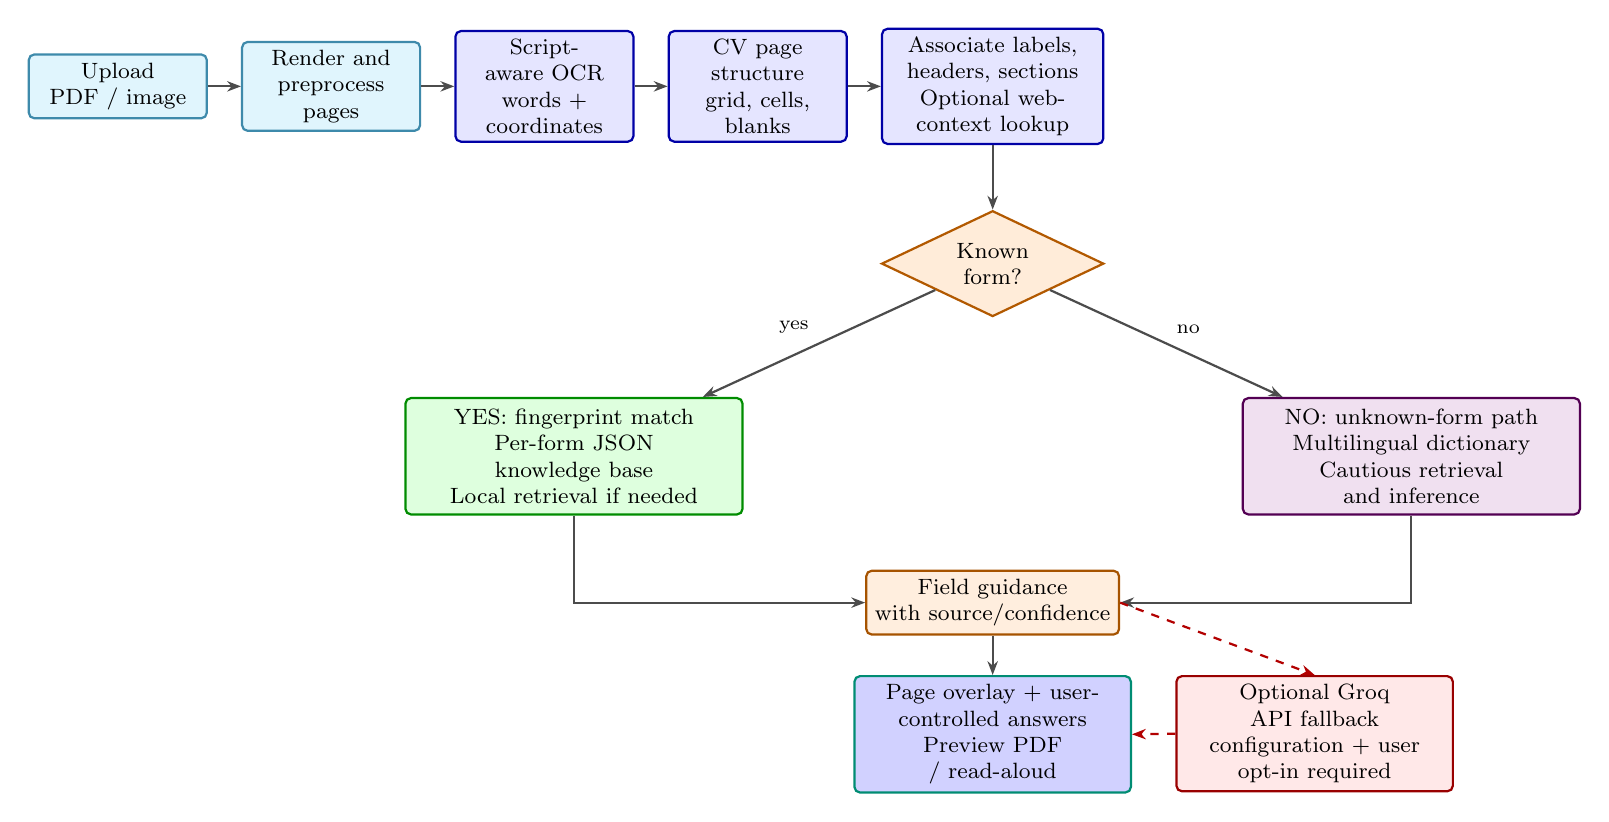
\begin{tikzpicture}[
  font=\footnotesize,
  node distance=0.35cm and 0.42cm,
  process/.style={rectangle, draw, rounded corners=2pt, thick,
                  align=center, text width=2.05cm, minimum height=0.76cm,
                  inner sep=3pt},
  branch/.style={rectangle, draw, rounded corners=2pt, thick,
                 align=center, text width=4.0cm, minimum height=0.88cm,
                 inner sep=4pt},
  decision/.style={diamond, draw=orange!70!black, fill=orange!15, thick,
                   align=center, aspect=2.1, text width=1.5cm, inner sep=1pt},
  arrow/.style={-{Stealth[length=5pt]}, thick, draw=black!70},
  optional/.style={-{Stealth[length=5pt]}, thick, dashed, draw=red!70!black}
]
  \node[process, fill=cyan!12, draw=cyan!65!black] (upload)
    {Upload\\PDF / image};
  \node[process, fill=cyan!12, draw=cyan!65!black, right=of upload] (prepare)
    {Render and\\preprocess pages};
  \node[process, fill=blue!10, draw=blue!65!black, right=of prepare] (ocr)
    {Script-aware OCR\\words + coordinates};
  \node[process, fill=blue!10, draw=blue!65!black, right=of ocr] (cv)
    {CV page structure\\grid, cells, blanks};
  \node[process, fill=blue!10, draw=blue!65!black, text width=2.6cm, right=of cv] (labels)
    {Associate labels, headers, sections\\Optional web-context lookup};
  \node[decision, below=0.82cm of labels] (knownq) {Known form?};
  \node[branch, fill=green!13, draw=green!55!black, below left=1.35cm and 2.45cm of knownq] (known)
    {YES: fingerprint match\\Per-form JSON knowledge base\\Local retrieval if needed};
  \node[branch, fill=violet!12, draw=violet!65!black, below right=1.35cm and 2.45cm of knownq] (unknown)
    {NO: unknown-form path\\Multilingual dictionary\\Cautious retrieval and inference};
  \node[process, fill=orange!13, draw=orange!65!black, below=3.2cm of knownq, text width=3.0cm] (merge)
    {Field guidance\\with source/confidence};
  \node[process, fill=blue!18, draw=green!55!blue, below=0.5cm of merge, text width=3.3cm] (user)
    {Page overlay + user-controlled answers\\Preview PDF / read-aloud};
  \node[process, fill=red!9, draw=red!60!black, below right=0.5cm and 0.7cm of merge, text width=3.3cm] (groq)
    {Optional Groq API fallback\\configuration + user opt-in required};

  \draw[arrow] (upload) -- (prepare);
  \draw[arrow] (prepare) -- (ocr);
  \draw[arrow] (ocr) -- (cv);
  \draw[arrow] (cv) -- (labels);
  \draw[arrow] (labels) -- (knownq);
  \draw[arrow] (knownq) -- node[above left, font=\scriptsize] {yes} (known);
  \draw[arrow] (knownq) -- node[above right, font=\scriptsize] {no} (unknown);
  \draw[arrow] (known.south) |- (merge.west);
  \draw[arrow] (unknown.south) |- (merge.east);
  \draw[arrow] (merge) -- (user);
  \draw[optional] (merge.east) -- (groq.north);
  \draw[optional] (groq.west) -- (user.east);
\end{tikzpicture}
\caption{End-to-end FormSathi process. The optional Groq compound-model search of webpages based on the printed title, issuing authority, and abbreviations is used as the background information at the label/context association step. The resulting information is provided to either form branch; it is not considered as an instruction of what the user should write. Known and unseen forms go through the same page rendering, OCR and computer vision procedures.}
\label{fig:architecture}
\end{figure*}

\subsection{External Groq Processing and Local Knowledge}
\label{sec:localarchitecture}

FormSathi has no local generative LLM and no local LLM decoder and generation layers to be specified. Its local language-related components include (i) per-form knowledge and a multilingual 56-concepts dictionary, (ii) exact, contained, and fuzzy-token matching, and (iii) sentence-transformer embedding model with ChromaDB/lexical retrieval in case of lack of exact match. The selected encoder is \texttt{paraphrase-multilingual-MiniLM-L12-v2}; it provides retrieval vectors, not a generative text output. Figure~\ref{fig:localstack} depicts the difference between local inference and optional Groq API call. There are no claims of specific number of internal layers of a nonexistent generative model.

\begin{figure*}[t]
\centering
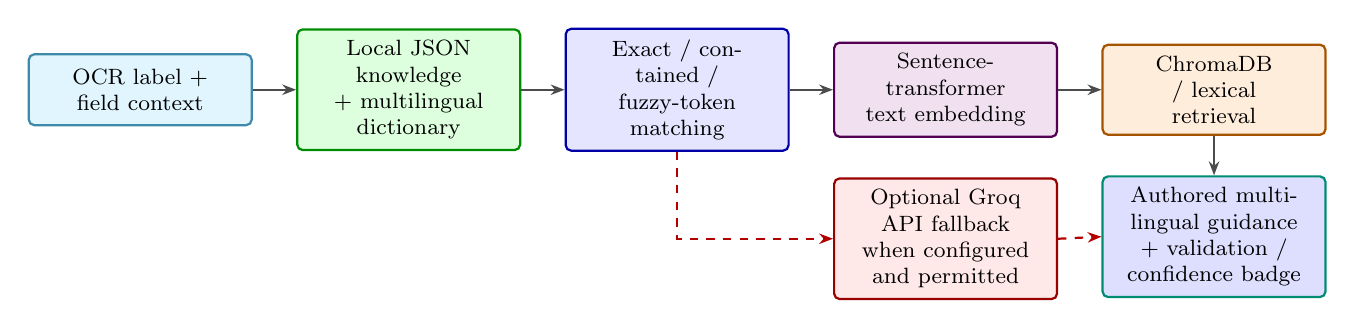
\begin{tikzpicture}[
  font=\footnotesize,
  node distance=0.38cm and 0.55cm,
  layer/.style={draw, rounded corners=2pt, thick, align=center,
                text width=2.55cm, minimum height=0.9cm, inner sep=4pt},
  arrow/.style={-{Stealth[length=5pt]}, thick, draw=black!70},
  remote/.style={-{Stealth[length=5pt]}, thick, dashed, draw=red!70!black}
]
  \node[layer, fill=cyan!12, draw=cyan!65!black] (input)
    {OCR label + field context};
  \node[layer, fill=green!13, draw=green!55!black, right=of input] (kb)
    {Local JSON knowledge\\+ multilingual dictionary};
  \node[layer, fill=blue!10, draw=blue!65!black, right=of kb] (match)
    {Exact / contained /\\fuzzy-token matching};
  \node[layer, fill=violet!12, draw=violet!65!black, right=of match] (embed)
    {Sentence-transformer\\text embedding};
  \node[layer, fill=orange!14, draw=orange!65!black, right=of embed] (retrieve)
    {ChromaDB / lexical\\retrieval};
  \node[layer, fill=blue!13, draw=green!55!blue, below=0.5cm of retrieve] (answer)
    {Authored multilingual guidance\\+ validation / confidence badge};
  \node[layer, fill=red!9, draw=red!60!black, below=0.5cm of embed] (groq)
    {Optional Groq API fallback\\when configured and permitted};

  \draw[arrow] (input) -- (kb);
  \draw[arrow] (kb) -- (match);
  \draw[arrow] (match) -- (embed);
  \draw[arrow] (embed) -- (retrieve);
  \draw[arrow] (retrieve) -- (answer);
  \draw[remote] (match.south) |- (groq.west);
  \draw[remote] (groq.east) -- (answer.west);
\end{tikzpicture}
\caption{Local knowledge stack and external fallback. The embedding model retrieves relevant text; it is not a generative LLM. The Groq call is made only along the dashed arrow and user-provided answers are not included in the request.}
\label{fig:localstack}
\end{figure*}

The form fingerprint determines whether the form is seen or unseen at the stage of field guidance resolution. A seen form will use its per-form field entry first; an unseen form relies on multilingual matching and higher retrieval threshold. In case of context-aware interpretation, page text is used to disambiguate labels and headers in either case. In case of lack of relevant local source, an external request is made only if the deployment configuration and user permissions allow it; otherwise the inference provides an explanation or unavailable message respectively.

\subsection{Frontend}

Frontend displays the processed page image with pixel-exact overlay elements over each blank field. On click, an in-place input appears and the text is centered and resized to keep it visible. Guidance panel displays the plain-language explanation in the selected language, with a button to hear it aloud. Language change of explanation is a local lookup: all four languages are provided in one API response, therefore no re-reading of the form happens and typed answers remain intact.

\subsection{Backend}

The backend is a FastAPI application. Key services are:
\begin{itemize}
  \item \textbf{PdfService}: renders PDF pages to PNG at 2$\times$ resolution; parses the embedded text layer if it is in correct format.
  \item \textbf{ImageService}: deskews, normalizes the contrast and optionally crops to form boundaries.
  \item \textbf{OCRService}: runs Tesseract with script detection; concatenates two OCR passes (rules-erased and rules-intact).
  \item \textbf{PageStructureService}: detects the ruled grids, generates cell locations and finds free-blanks.
  \item \textbf{FieldAssemblyService}: combines structural blanks with shape detector candidates.
  \item \textbf{FieldSemanticsService}: performs matching of labels against multilingual dictionary.
  \item \textbf{GuidanceService}: retrieves and formats the guidance from knowledge base.
\end{itemize}

% ------------------------------------------------------------------
\section{Page Structure Service}
\label{sec:pagestructure}

The page-structure service is the main innovation behind FormSathi, compared to the approach based only on OCR. The service's development was motivated by the observed failure cases: a simple box detector applied to the ECI Annexure-IV form detected 121 rectangles, retained the outer border of the table and removed all cells inside it, resulting in 2 fields out of a total of 30 fields.

\subsection{Ruled-Grid Recovery}

The service detects horizontal and vertical ink lines using morphological opening, dilates them to close scan breaks and intersects to obtain cells as rectangular areas. The cell smaller than 24$\times$14 pixels is considered to be a rule artifact. Cells that share the same row header are flagged; the rest of the cells become fields.

\subsection{Caption-and-Blank Cohabitation}

Many government forms print a caption and its corresponding blank in one cell: \texttt{Elector Name: \_\_\_\_\_}. A cell whose OCR text ends with a colon, and whose right part (at least 35\% of the cell width) is ink-free, results in an \textit{inline blank}, which is placed at the free area.

\subsection{Free-Standing Caption Detection}

In unruled forms, captions ending with a colon and occupying less than 60\% of the page width are considered invitations for writing. In this case, the blank is the area to the right (or left, for right-to-left pages).

\subsection{Dotted-Leader Blank Detection}
\label{sec:dotleaders}
In PDF native government forms, such as the passport parent-declaration annexures, the fill-in space is printed as a run of dot or ellipsis characters merged with the caption into one PDF word: \texttt{Date of Birth:......}. This structure is invisible for a colon gap detector and does not produce any ink rule for a morphological detector to detect.

For each text line the service searches the longest run of periods, ellipses, middle dots, bullets, underscores, and similar leader characters that are present at least for three consecutive characters. Caption is the text before the run (without trailing leader characters); the blank occupies the pixel width of the leader run. If two leader runs are found in one text line, the service creates two separate fields for these runs, allowing father and mother columns in a single line.

If the prefix of the mid-sentence leader is a stop word ("of", "the", "to", and so forth), the parenthetical text after the dots serves as the caption: \texttt{of...(name of the minor child)} will yield the caption \textit{name of the minor child}.

Previously, pure leader PDF words without alphabetic characters were filtered out during the text-layer processing. The filter was improved to keep any word having leader-character count of at least 3.

\subsection{Prose Detection}

An instruction sheet should not be treated like a form. A service considers a page to be a prose page in case: (i) there is no grid on the page; (ii) there are at least 8 text lines; and (iii) either the median line width is larger than 60\% of the widest line or at least 4 lines are wider than 42\% of the page width. Pages with at least 2 lines with a short colon-caption are never regarded as prose pages.

Dotted leader lines break the prose gate --- each line contains its own writing area and is extracted prior to prose gate evaluation.

\subsection{Overlap Suppression}

Each suggested blank is checked against all words in the OCR result. Blank that partially or fully overlaps with printed word is ignored: a blank is something to write, and hence is something that is not written yet.

% ------------------------------------------------------------------
\section{Field Understanding and Multilingual Guidance}
\label{sec:understanding}

\subsection{Multilingual Field Dictionary}

The common-field dictionary includes 56 fields and 927 wordings in English, Hindi, Kannada and Urdu. Each entry contains: canonical identifier; aliases in all 4 scripts; validation type (date, mobile, PAN, IFSC, amount, name, text, \dots); plain-language \textit{what to enter} and \textit{why needed} text in native script; and an example in native script.

All multilingual strings are authored manually. Translation services are not used at run-time.

\subsection{Three-Tier Matching}

Given a printed label, matching is done in order of decreasing confidence:
\begin{enumerate}
  \item \textbf{Exact}: the folded label in the script-sensitive way equals a folded alias.
  \item \textbf{Contained}: the alias is fully contained in the label, or vice versa, and the shorter word explains at least half of the meaning of the longer.
  \item \textbf{Fuzzy token}: the ratio of tokens in the label that correspond to tokens in the alias (based on Jaro-Winkler similarity metric) exceeds a floor value specific for the tier.
\end{enumerate}

Tiers 1 and 2 give confident guidance; tier 3 gives the guidance that should be verified by user. Every step from tier 1 is presented to the user as part of the UI so he could understand how much the system trusts the guidance.

\subsection{Resolution Ladder}

Sources of guidance are taken into account in the order given in Table~\ref{tab:resolution}. Contextual interpretation of a page is available only in case it is configured; generation of a field by external field generator additionally requires user consent.

\begin{table}[htbp]
\caption{FormSathi Resolution Ladder}
\label{tab:resolution}
\centering
\footnotesize
\begin{tabularx}{\columnwidth}{@{}p{0.25\columnwidth}X p{0.27\columnwidth}@{}}
\toprule
\textbf{Source} & \textbf{When used} & \textbf{UI indicator} \\
\midrule
Known-form KB & Recognised fingerprint and matching field & Known Form KB \\
Page context & Configured contextual interpretation resolves field & Read From Page \\
Common dictionary & Exact or contained wording match & Common Dictionary \\
Plausible dictionary & Fuzzy match; verification needed & Common Dictionary (verify) \\
Local retrieval & Relevant result cleared the threshold & Retrieved Guidance (verify) \\
Groq API & Configured and explicitly allowed & AI Guidance (verify) \\
Label pattern & Only answer shape can be inferred & Inferred \\
Unavailable & No interpretation supported & Guidance unavailable \\
\bottomrule
\end{tabularx}
\end{table}

\subsection{Known-Form Knowledge Base and RAG}

For a recognised known form, FormSathi checks for its fields in a per-form JSON entry. Failing both the known form and page-context interpretation, it attempts exact, contained, and fuzzy-token matches to the common-field dictionary. Retrieval uses the multilingual sentence embedding and ChromaDB for the more demanding case of unknown form; there is also an option for lexical retrieval \cite{rag}. Retrieved chunks keep the source metadata. This is the local retrieval and matching step, not the local text generation.

\subsection{Known and Unknown Form Paths}

The shared computer-vision path prepares each page, obtains OCR text and word coordinates, recovers ruled cells and other candidate blanks, associates labels with fields, and retains nearby headers and section context. Form fingerprinting selects the known or unknown case. A recognised known form uses its curated field record first. For either case, configured page-context interpretation can resolve a field before dictionary matching. Remaining unknown fields use the four-script common dictionary and then local retrieval at the higher unknown-form threshold; if neither applies, the configured Groq API may interpret the printed label only when the user has allowed external AI. A label-pattern rule can describe the answer's shape without claiming an unsupported definition; otherwise guidance is unavailable. All sources return to the same multilingual UI, validation, field overlay, and reference-preview workflow.

The known-form fingerprint matcher scores each candidate form on the fraction of its fingerprint terms found in the full-page OCR text (weight 0.55), the fraction of its field aliases that appear in detected labels (weight 0.40), and a category bonus (0.12 for a matching category), capped at 1.0. The configured recognition threshold is 0.42.

\subsection{Context-Aware Page Interpretation}

Page-level interpretation for configured external AI fetches a title, purpose, glossary, and completion context from the printed text. Field-level requests include caption, column header, section header, and that page context; this allows to distinguish between identical labels in various contexts and interpret abbreviations like \textit{AC Name}. Requests are batched by the implementation in order to limit the response size.

The external model is fed text rather than page images or user-entered answers. Answer generated by it is discarded if it is not written in the requested script; thus, rejected output leads to a local inference or unavailable state. This project does not have any locally hosted generative model.

\subsection{Per-Field Validation}

Each field has a validation rule derived from its semantic identifier. The kinds supported are date (DD/MM/YYYY with regional digit acceptances), Indian mobile, PIN code, Aadhaar, PAN, IFSC, bank account, email, amount, year, and name. Messages of validation are authored in all four languages.

% ------------------------------------------------------------------
\section{Implementation}
\label{sec:implementation}

\subsection{Technology Stack}

\begin{itemize}
  \item \textbf{Frontend}: React 18, TypeScript, Vite, Tailwind CSS, Vitest (about 38 tests).
  \item \textbf{Backend}: FastAPI, Pydantic v2, OpenCV, Pillow, PyMuPDF, Tesseract 5, SQLite, ChromaDB, Sentence Transformers, HarfBuzz/FreeType (Indic text shaping in previews) \cite{fastapi,opencv,pymupdf,chroma,sentence_transformers,harfbuzz}.
  \item \textbf{Generative model}: optional external Groq OpenAI-compatible API; enabled only if configured and permitted. No local generative LLM is deployed.
  \item \textbf{Voice}: ElevenLabs multilingual-v3 (falls back to browser speech synthesis).
\end{itemize}

\subsection{Script-Aware OCR}

The service first determines the dominant Unicode block among the page text, and then uses Tesseract with the corresponding language model and the English language model \cite{tesseract,multilingual_ocr}. This allows us to load alphabets one-by-one, but retain cross-script glyphs (like the Kannada \textit{EPIC} in the Latin script).

Two passes are made per page: with rules removed (to make letters behind the rules readable), and with rules intact (so that the rule is not misinterpreted as a blank line). The results of these passes are merged word-by-word based on confidence, preferring the higher-confidence reading at every point.

\subsection{Reference Preview Generation}

The user-typed answers are rendered back onto the image using HarfBuzz and FreeType, that accurately shape Devanagari, Kannada and Urdu (right-to-left script). Each answer is resized to fit completely into its blank. The preview is outputted as a PDF for the user to print out as a reference when completing the official form manually.

\subsection{Privacy Design}

User-typed answers are stored in the browser state and sent to the backend only when the user requests the preview rendering. They are never transmitted to the external LLM. The external model gets only the text from the printed form. CORS access is restricted to whitelisted origins. Uploads get server-side-generated UUID filenames. 

\subsection{Reliability Controls}

A circuit breaker suspends the optional LLM after three failures in a row and resumes after some cooldown time. Failed batches are bisected and partially recovered. Up to two whitelisted API keys and the LLM / fallback model sequence can be tried in case of rate limits or server errors. Results are cached by page structure hash.

% ------------------------------------------------------------------
\section{Experimental Evaluation}
\label{sec:evaluation}

\subsection{Evaluation Setup}

We supply two artifacts with the committed evaluation results. The pipeline evaluation has four seeded known-form images and five unknown-form images; the unknown-flow evaluation has four synthetic form templates in English, Hindi, Kannada and Urdu, each of them rendered as \textit{clean} and \textit{noisy} images (15-degree rotation, Gaussian blur, 70\% brightness and salt-and-pepper noise). All unknown-flow images have nine ground-truth fields. The ground truth was obtained from the sample generation scripts in the repository. Field box precision, recall and F1 were measured with IoU = 0.3 threshold. The unknown-flow semantic measure checks that all expected canonical field identifiers were found.

Metrics:
\begin{itemize}
  \item \textbf{Field-box recall}: fraction of ground-truth fields for which a blank overlapping the true region is detected.
  \item \textbf{Semantic recall}: fraction of ground-truth fields correctly resolved to their dictionary identifier.
\end{itemize}

\subsection{Field Detection Results}

\begin{table}[htbp]
\caption{Field-Box Recall for Known and Unknown Forms}
\label{tab:detection}
\centering
\footnotesize
\begin{tabular}{@{}llccc@{}}
\toprule
\textbf{Form group} & \textbf{Case} & \textbf{Found} & \textbf{Total} & \textbf{Recall} \\
\midrule
Known & 4 seeded images & 28 & 28 & 1.00 \\
\midrule
Unknown English & Clean & 9 & 9 & 1.00 \\
Unknown English & Noisy & 9 & 9 & 1.00 \\
Unknown Hindi & Clean & 9 & 9 & 1.00 \\
Unknown Hindi & Noisy & 9 & 9 & 1.00 \\
Unknown Kannada & Clean & 9 & 9 & 1.00 \\
Unknown Kannada & Noisy & 9 & 9 & 1.00 \\
Unknown Urdu & Clean & 9 & 9 & 1.00 \\
Unknown Urdu & Noisy & 9 & 9 & 1.00 \\
\midrule
\multicolumn{3}{l}{\textbf{Unknown-flow total}} & \textbf{72} & \textbf{1.00} \\
\bottomrule
\end{tabular}
\end{table}

The field-box recall is 1.00 for 28 ground-truth fields in known-form images and for all 72 fields in eight unknown-flow image variants. These numbers characterize the provided synthetic test set, not the expected performance on arbitrary real forms.

\subsection{Semantic Resolution Results}

\begin{table}[htbp]
\caption{Semantic Recall by Language and Variant}
\label{tab:semantic}
\centering
\footnotesize
\begin{tabular}{@{}llccc@{}}
\toprule
\textbf{Language} & \textbf{Variant} & \textbf{Resolved} & \textbf{Total} & \textbf{Recall} \\
% \midrule
% Known forms & Not measured & -- & -- & -- \\
\midrule
English  & Clean & 9 & 9 & 1.00 \\
English  & Noisy & 9 & 9 & 1.00 \\
Hindi    & Clean & 9 & 9 & 1.00 \\
Hindi    & Noisy & 9 & 9 & 1.00 \\
Kannada  & Clean & 8 & 9 & 0.89 \\
Kannada  & Noisy & 9 & 9 & 1.00 \\
Urdu     & Clean & 6 & 9 & 0.67 \\
Urdu     & Noisy & 6 & 9 & 0.67 \\
\midrule
\multicolumn{2}{l}{\textbf{Unknown-flow total}} & \textbf{65} & \textbf{72} & \textbf{0.90} \\
\bottomrule
\end{tabular}
\end{table}

The semantic recall is not reported for the known-form group because the committed known-form evaluation tests the field localization and form fingerprinting, but not the accuracy of canonical meanings. In the unknown-form group, English and Hindi get 9/9 on both variants; Kannada scores 8/9 and 9/9 on clean and noisy inputs respectively; Urdu gets 6/9 on each variant. The errors in semantic recall do not separate OCR errors from downstream ones, hence these misses cannot be blamed on a particular component alone.

The unknown-flow script check looked at 87 detected fields in four guidance languages (348 field-language outputs). There were zero missing-language outputs and zero wrong-script outputs in the recorded run. This check concerns generated guidance outputs only, not user understanding or factual accuracy.

\subsection{Multilingual Script Fidelity}

Guidance text is authored in the target scripts instead of machine translation. The optional LLM text is independently validated for the target script. Neither property ensures factual accuracy; human validation is still required for that measure.

\subsection{Known-Form Identification}

Table~\ref{tab:formid} reports the decisions recorded by the pipeline evaluation.

\begin{table}[htbp]
\caption{Known-Form Recognition and Unknown-Form Rejection}
\label{tab:formid}
\centering
\footnotesize
\begin{tabular}{@{}lccc@{}}
\toprule
\textbf{Group} & \textbf{Correct decisions} & \textbf{Total} & \textbf{Rate} \\
\midrule
Known seeded forms & 4 & 4 & 1.00 \\
Unknown forms correctly rejected & 5 & 5 & 1.00 \\
\bottomrule
\end{tabular}
\end{table}

The five unknown-form identification images are the samples in \texttt{evaluation\_results.json}; the eight clean/noisy language combinations in the separate unknown flow are not additional identification trials. Raw known-form fingerprint scores are not present in the saved JSON file, so there is no per-form score claimed here.

\begin{table}[htbp]
\caption{Pipeline Metrics by Form Group}
\label{tab:groups}
\centering
\footnotesize
\begin{tabular}{@{}lccccc@{}}
\toprule
\textbf{Group} & \textbf{Samples} & \textbf{Precision} & \textbf{Recall} & \textbf{F1} & \textbf{Time (s)} \\
\midrule
Known forms & 4 & 0.938 & 1.000 & 0.967 & 3.84 \\
Unknown forms & 5 & 0.874 & 1.000 & 0.930 & 4.83 \\
\bottomrule
\end{tabular}
\end{table}

Table~\ref{tab:groups} shows unweighted means across the per-image values in \texttt{evaluation\_results.json}; time represents the mean time per image in that run. This is not a controlled experiment of model family and hardware setup comparisons.

\subsection{Test Coverage}

The automated tests in the repository cover page structure, form analysis, multilingual dictionary, label association (with right-to-left text), pipeline integration, validity check, and dotted-leader detection. Counts of test pass results are not reported as performance measures of the research system.

% ------------------------------------------------------------------
\section{Discussion}

\subsection{Design Choices}

\textbf{Authoring multilingual strings instead of machine translation}. While machine translation of the guidance text would enable quick extension into more languages, it opens up two possible failure modes: misuse of technical terms in the target language, and generation of an answer in the mixed or incorrect script. Authoring strings solves both problems at the expense of manual labor per language.

\textbf{Structural detection instead of pure deep learning}. While learned models such as LayoutLM or Donut are capable of producing joint text/layout representation, they require pretrained model weights and inference time. FormSathi's deterministic page structure service is meant for CPU usage and explainability: every blank is generated by a particular cell, dotted-leader, or caption-gap rule.

\textbf{Privacy by design}. Answer data stays in the browser during the form fill process and only moves to the backend when a user makes a request for a reference render of the form with those answers. No information is ever sent to Groq, thus preventing the forward of personal answers to an external model while maintaining the need to trust the deployment receiving the reference render request.

\subsection{Limitations}

Urdu semantic recall is the lowest among all of the synthetic sample languages, however the measurements cannot separate OCR errors from errors in matching. Current local OCR implementation is based on Tesseract and has not been tested against the vision-language OCR. An external vision model would also change the privacy assumptions of the deployment.

The field dictionary contains definitions for 56 concepts. Forms using terminology not included in the field dictionary would get an inferred description of the answer shape instead of a definition. Synthetic forms created by the same author as the generator were used for the evaluation and do not include any judgments of explanation accuracy, task completeness, or usability. The literature search also involved one reviewer and one repository, so it should not be viewed as a systematic review.

% ------------------------------------------------------------------
\section{Conclusion}
\label{sec:conclusion}

FormSathi is a hybrid computer vision and retrieval system for multilingual form assistance. Committed evaluation shows 1.00 field-box recall on known and synthetic unknown samples, and 0.90 semantic recall on 72 unknown-form fields. The samples are project-generated and small, rather than evidence of general performance. Grid recovery, authoring multilingual strings, source/confidence indicators, and privacy-aware handling form the foundation of the system.

Dotted-leader detection feature allows the system to be used with the PDF-native form annexes where the fill-in spaces are represented as typographic leader characters, rather than empty boxes or ruled lines. Parenthetical captions recovery enables mid-sentence leaders where captions are printed after the dots.

Future directions include experiments with externally collected forms, confidence calibration, human-rater evaluation of guidance accuracy and time to complete the task, field dictionary expansion, and comparison between Tesseract-based OCR and alternative multilingual OCR services.

% ------------------------------------------------------------------
% ------------------------------------------------------------------
\begin{thebibliography}{00}

\bibitem{prisma2020}
M.\ J.\ Page \textit{et al.}, ``The PRISMA 2020 statement: An updated guideline for reporting systematic reviews,'' \textit{BMJ}, vol.~372, p.~n71, 2021, doi: 10.1136/bmj.n71.

\bibitem{funsd}
G.\ Jaume, H.\ K.\ Ekenel, and J.-P.\ Thiran, ``FUNSD: A dataset for form understanding in noisy scanned documents,'' in \textit{Proc.\ Int.\ Conf.\ Document Analysis and Recognition Workshops (ICDARW)}, 2019. [Online]. Available: \url{https://arxiv.org/abs/1905.13538}

\bibitem{tesseract}
R.\ Smith, ``An overview of the Tesseract OCR engine,'' in \textit{Proc.\ 9th Int.\ Conf.\ Document Analysis and Recognition (ICDAR)}, 2007, pp.~629--633.

\bibitem{layoutlm}
Y.\ Xu, M.\ Li, L.\ Cui, S.\ Huang, F.\ Wei, and M.\ Zhou, ``LayoutLM: Pre-training of text and layout for document image understanding,'' in \textit{Proc.\ 26th ACM SIGKDD Int.\ Conf.\ Knowledge Discovery \& Data Mining}, 2020, pp.~1192--1200.

\bibitem{rag}
P.\ Lewis, E.\ Perez, A.\ Piktus, F.\ Petroni, V.\ Karpukhin, N.\ Goyal, H.\ K\"uttler, M.\ Lewis, W.\ Yih, T.\ Rockt\"aschel, S.\ Riedel, and D.\ Kiela, ``Retrieval-augmented generation for knowledge-intensive NLP tasks,'' in \textit{Advances in Neural Information Processing Systems (NeurIPS)}, vol.~33, 2020, pp.~9459--9474.

\bibitem{donut}
G.\ Kim \textit{et al.}, ``OCR-free document understanding transformer,'' in \textit{Proc.\ European Conf.\ Computer Vision (ECCV)}, 2022, pp.~498--517.

\bibitem{chroma}
Chroma, ``Chroma documentation.'' [Online]. Available: \url{https://docs.trychroma.com/}

\bibitem{sentence_transformers}
N.\ Reimers and I.\ Gurevych, ``Sentence-BERT: Sentence embeddings using siamese BERT-networks,'' in \textit{Proc.\ 2019 Conf.\ Empirical Methods in Natural Language Processing (EMNLP)}, 2019, pp.~3982--3992.

\bibitem{fastapi}
S.\ Ram\'irez, ``FastAPI,'' 2019. [Online]. Available: \url{https://fastapi.tiangolo.com}

\bibitem{pymupdf}
``PyMuPDF: Python bindings for MuPDF,'' Artifex Software, 2024. [Online]. Available: \url{https://pymupdf.readthedocs.io}

\bibitem{opencv}
G.\ Bradski, ``The OpenCV library,'' \textit{Dr.\ Dobb's Journal of Software Tools}, 2000.

\bibitem{harfbuzz}
B.\ Esfahbod, ``HarfBuzz: An OpenType text shaping engine,'' 2012. [Online]. Available: \url{https://harfbuzz.github.io}

\bibitem{formnet}
C.-Y.\ Lee \textit{et al.}, ``FormNet: Structural encoding beyond sequential modeling in form document information extraction,'' 2022. [Online]. Available: \url{https://arxiv.org/abs/2203.08411}

\bibitem{layoutlmv3}
Y.\ Huang, T.\ Lv, L.\ Cui, Y.\ Lu, and F.\ Wei, ``LayoutLMv3: Pre-training for document AI with unified text and image masking,'' in \textit{Proc.\ ACM Int.\ Conf.\ Multimedia}, 2022. [Online]. Available: \url{https://arxiv.org/abs/2204.08387}

\bibitem{formnetv2}
C.-Y.\ Lee \textit{et al.}, ``FormNetV2: Multimodal graph contrastive learning for form document information extraction,'' 2023. [Online]. Available: \url{https://arxiv.org/abs/2305.02549}

\bibitem{multilingual_ocr}
J.\ Huang \textit{et al.}, ``A multiplexed network for end-to-end, multilingual OCR,'' 2021. [Online]. Available: \url{https://arxiv.org/abs/2103.15992}

\bibitem{form_attacks}
M.\ Gao, Z.\ Chen, C.\ Xiong, and R.\ Xu, ``Robustness evaluation of transformer-based form field extractors via form attacks,'' 2021. [Online]. Available: \url{https://arxiv.org/abs/2110.04413}

\bibitem{formfactory}
B.\ Li \textit{et al.}, ``FormFactory: An interactive benchmarking suite for multimodal form-filling agents,'' 2025. [Online]. Available: \url{https://arxiv.org/abs/2506.01520}

\end{thebibliography}

\end{document}
